% Created by tikzDevice version 0.10.1 on 2020-02-15 16:09:02
% !TEX encoding = UTF-8 Unicode
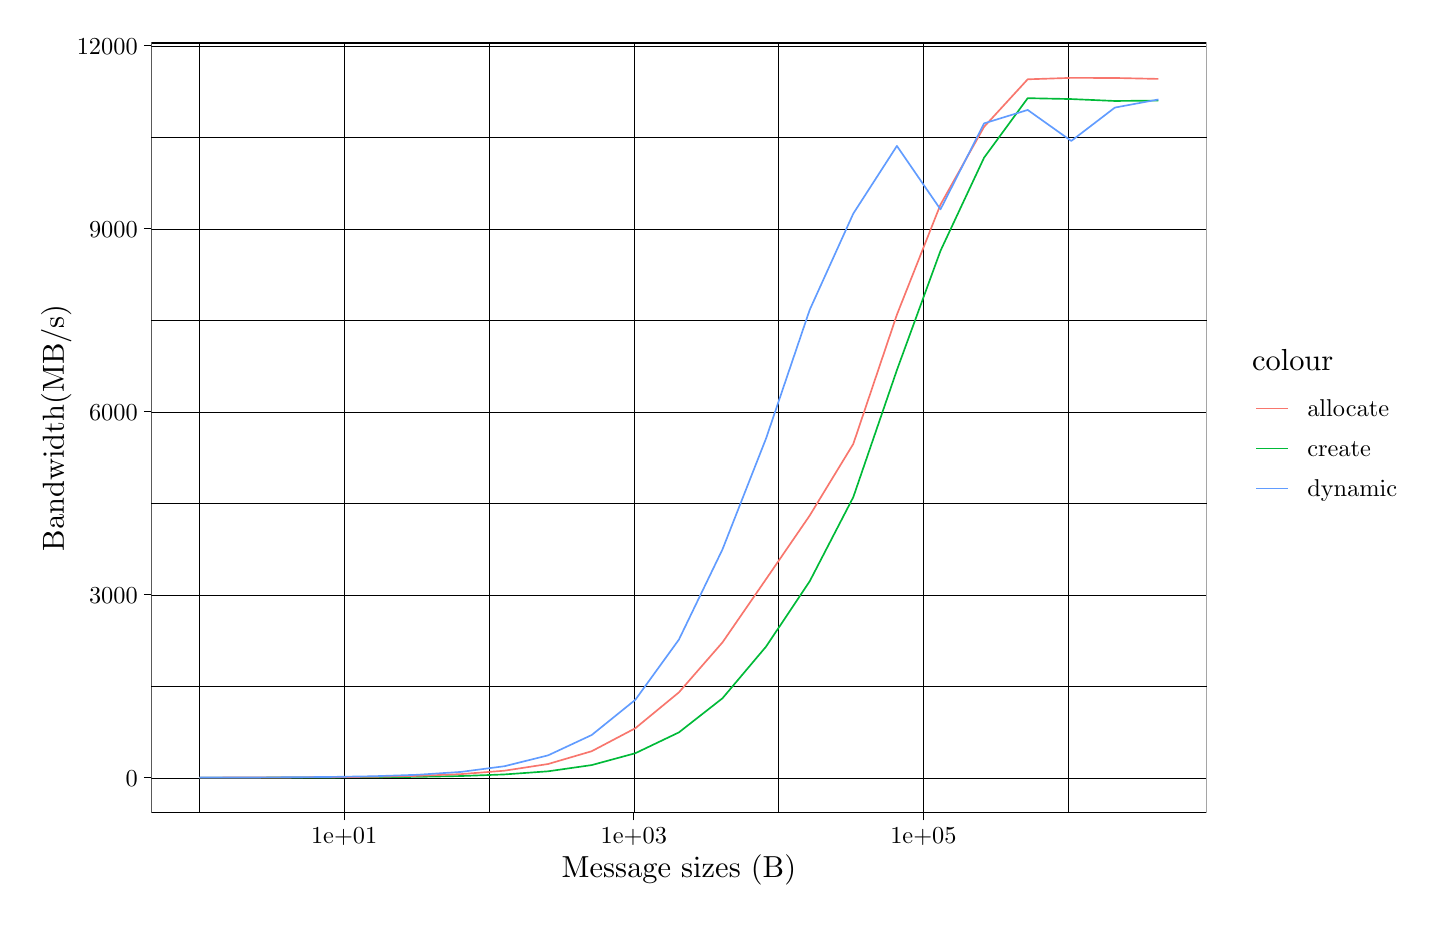
\begin{tikzpicture}[x=1pt,y=1pt]
\definecolor{fillColor}{RGB}{255,255,255}
\path[use as bounding box,fill=fillColor,fill opacity=0.00] (0,0) rectangle (505.89,314.37);
\begin{scope}
\path[clip] (  0.00,  0.00) rectangle (505.89,314.37);
\definecolor{drawColor}{RGB}{255,255,255}
\definecolor{fillColor}{RGB}{255,255,255}

\path[draw=drawColor,line width= 0.6pt,line join=round,line cap=round,fill=fillColor] (  0.00,  0.00) rectangle (505.89,314.37);
\end{scope}
\begin{scope}
\path[clip] ( 44.71, 30.72) rectangle (425.93,308.87);
\definecolor{fillColor}{RGB}{255,255,255}

\path[fill=fillColor] ( 44.71, 30.72) rectangle (425.93,308.87);
\definecolor{drawColor}{RGB}{0,0,0}

\path[draw=drawColor,line width= 0.0pt,line join=round] ( 44.71, 76.42) --
	(425.93, 76.42);

\path[draw=drawColor,line width= 0.0pt,line join=round] ( 44.71,142.55) --
	(425.93,142.55);

\path[draw=drawColor,line width= 0.0pt,line join=round] ( 44.71,208.67) --
	(425.93,208.67);

\path[draw=drawColor,line width= 0.0pt,line join=round] ( 44.71,274.80) --
	(425.93,274.80);

\path[draw=drawColor,line width= 0.0pt,line join=round] ( 62.04, 30.72) --
	( 62.04,308.87);

\path[draw=drawColor,line width= 0.0pt,line join=round] (166.70, 30.72) --
	(166.70,308.87);

\path[draw=drawColor,line width= 0.0pt,line join=round] (271.36, 30.72) --
	(271.36,308.87);

\path[draw=drawColor,line width= 0.0pt,line join=round] (376.02, 30.72) --
	(376.02,308.87);

\path[draw=drawColor,line width= 0.1pt,line join=round] ( 44.71, 43.36) --
	(425.93, 43.36);

\path[draw=drawColor,line width= 0.1pt,line join=round] ( 44.71,109.48) --
	(425.93,109.48);

\path[draw=drawColor,line width= 0.1pt,line join=round] ( 44.71,175.61) --
	(425.93,175.61);

\path[draw=drawColor,line width= 0.1pt,line join=round] ( 44.71,241.73) --
	(425.93,241.73);

\path[draw=drawColor,line width= 0.1pt,line join=round] ( 44.71,307.86) --
	(425.93,307.86);

\path[draw=drawColor,line width= 0.1pt,line join=round] (114.37, 30.72) --
	(114.37,308.87);

\path[draw=drawColor,line width= 0.1pt,line join=round] (219.03, 30.72) --
	(219.03,308.87);

\path[draw=drawColor,line width= 0.1pt,line join=round] (323.69, 30.72) --
	(323.69,308.87);
\definecolor{drawColor}{RGB}{0,186,56}

\path[draw=drawColor,line width= 0.6pt,line join=round] ( 62.04, 43.37) --
	( 77.80, 43.38) --
	( 93.55, 43.40) --
	(109.30, 43.43) --
	(125.05, 43.51) --
	(140.81, 43.65) --
	(156.56, 43.95) --
	(172.31, 44.53) --
	(188.07, 45.66) --
	(203.82, 47.91) --
	(219.57, 52.19) --
	(235.32, 59.72) --
	(251.08, 72.06) --
	(266.83, 90.74) --
	(282.58,114.31) --
	(298.33,144.72) --
	(314.09,190.64) --
	(329.84,233.73) --
	(345.59,267.39) --
	(361.35,288.89) --
	(377.10,288.57) --
	(392.85,287.88) --
	(408.60,288.02);
\definecolor{drawColor}{RGB}{248,118,109}

\path[draw=drawColor,line width= 0.6pt,line join=round] ( 62.04, 43.38) --
	( 77.80, 43.40) --
	( 93.55, 43.44) --
	(109.30, 43.52) --
	(125.05, 43.68) --
	(140.81, 44.00) --
	(156.56, 44.64) --
	(172.31, 45.88) --
	(188.07, 48.30) --
	(203.82, 52.92) --
	(219.57, 61.22) --
	(235.32, 74.18) --
	(251.08, 92.26) --
	(266.83,115.12) --
	(282.58,138.07) --
	(298.33,163.95) --
	(314.09,210.65) --
	(329.84,250.43) --
	(345.59,278.53) --
	(361.35,295.71) --
	(377.10,296.23) --
	(392.85,296.19) --
	(408.60,295.85);
\definecolor{drawColor}{RGB}{97,156,255}

\path[draw=drawColor,line width= 0.6pt,line join=round] ( 62.04, 43.39) --
	( 77.80, 43.42) --
	( 93.55, 43.49) --
	(109.30, 43.62) --
	(125.05, 43.88) --
	(140.81, 44.40) --
	(156.56, 45.44) --
	(172.31, 47.50) --
	(188.07, 51.43) --
	(203.82, 58.78) --
	(219.57, 71.49) --
	(235.32, 93.25) --
	(251.08,125.88) --
	(266.83,165.98) --
	(282.58,212.40) --
	(298.33,247.18) --
	(314.09,271.63) --
	(329.84,248.71) --
	(345.59,279.78) --
	(361.35,284.64) --
	(377.10,273.44) --
	(392.85,285.49) --
	(408.60,288.42);
\definecolor{drawColor}{RGB}{0,0,0}

\path[draw=drawColor,line width= 0.6pt,line join=round,line cap=round] ( 44.71, 30.72) rectangle (425.93,308.87);
\end{scope}
\begin{scope}
\path[clip] (  0.00,  0.00) rectangle (505.89,314.37);
\definecolor{drawColor}{RGB}{0,0,0}

\node[text=drawColor,anchor=base east,inner sep=0pt, outer sep=0pt, scale=  0.88] at ( 39.76, 40.33) {0};

\node[text=drawColor,anchor=base east,inner sep=0pt, outer sep=0pt, scale=  0.88] at ( 39.76,106.45) {3000};

\node[text=drawColor,anchor=base east,inner sep=0pt, outer sep=0pt, scale=  0.88] at ( 39.76,172.58) {6000};

\node[text=drawColor,anchor=base east,inner sep=0pt, outer sep=0pt, scale=  0.88] at ( 39.76,238.70) {9000};

\node[text=drawColor,anchor=base east,inner sep=0pt, outer sep=0pt, scale=  0.88] at ( 39.76,304.83) {12000};
\end{scope}
\begin{scope}
\path[clip] (  0.00,  0.00) rectangle (505.89,314.37);
\definecolor{drawColor}{RGB}{0,0,0}

\path[draw=drawColor,line width= 0.3pt,line join=round] ( 41.96, 43.36) --
	( 44.71, 43.36);

\path[draw=drawColor,line width= 0.3pt,line join=round] ( 41.96,109.48) --
	( 44.71,109.48);

\path[draw=drawColor,line width= 0.3pt,line join=round] ( 41.96,175.61) --
	( 44.71,175.61);

\path[draw=drawColor,line width= 0.3pt,line join=round] ( 41.96,241.73) --
	( 44.71,241.73);

\path[draw=drawColor,line width= 0.3pt,line join=round] ( 41.96,307.86) --
	( 44.71,307.86);
\end{scope}
\begin{scope}
\path[clip] (  0.00,  0.00) rectangle (505.89,314.37);
\definecolor{drawColor}{RGB}{0,0,0}

\path[draw=drawColor,line width= 0.3pt,line join=round] (114.37, 27.97) --
	(114.37, 30.72);

\path[draw=drawColor,line width= 0.3pt,line join=round] (219.03, 27.97) --
	(219.03, 30.72);

\path[draw=drawColor,line width= 0.3pt,line join=round] (323.69, 27.97) --
	(323.69, 30.72);
\end{scope}
\begin{scope}
\path[clip] (  0.00,  0.00) rectangle (505.89,314.37);
\definecolor{drawColor}{RGB}{0,0,0}

\node[text=drawColor,anchor=base,inner sep=0pt, outer sep=0pt, scale=  0.88] at (114.37, 19.71) {1e+01};

\node[text=drawColor,anchor=base,inner sep=0pt, outer sep=0pt, scale=  0.88] at (219.03, 19.71) {1e+03};

\node[text=drawColor,anchor=base,inner sep=0pt, outer sep=0pt, scale=  0.88] at (323.69, 19.71) {1e+05};
\end{scope}
\begin{scope}
\path[clip] (  0.00,  0.00) rectangle (505.89,314.37);
\definecolor{drawColor}{RGB}{0,0,0}

\node[text=drawColor,anchor=base,inner sep=0pt, outer sep=0pt, scale=  1.10] at (235.32,  7.44) {Message sizes (B)};
\end{scope}
\begin{scope}
\path[clip] (  0.00,  0.00) rectangle (505.89,314.37);
\definecolor{drawColor}{RGB}{0,0,0}

\node[text=drawColor,rotate= 90.00,anchor=base,inner sep=0pt, outer sep=0pt, scale=  1.10] at ( 13.08,169.80) {Bandwidth(MB/s)};
\end{scope}
\begin{scope}
\path[clip] (  0.00,  0.00) rectangle (505.89,314.37);
\definecolor{fillColor}{RGB}{255,255,255}

\path[fill=fillColor] (436.93,135.11) rectangle (500.39,204.49);
\end{scope}
\begin{scope}
\path[clip] (  0.00,  0.00) rectangle (505.89,314.37);
\definecolor{drawColor}{RGB}{0,0,0}

\node[text=drawColor,anchor=base west,inner sep=0pt, outer sep=0pt, scale=  1.10] at (442.43,190.44) {colour};
\end{scope}
\begin{scope}
\path[clip] (  0.00,  0.00) rectangle (505.89,314.37);
\definecolor{fillColor}{RGB}{255,255,255}

\path[fill=fillColor] (442.43,169.52) rectangle (456.89,183.97);
\end{scope}
\begin{scope}
\path[clip] (  0.00,  0.00) rectangle (505.89,314.37);
\definecolor{drawColor}{RGB}{248,118,109}

\path[draw=drawColor,line width= 0.6pt,line join=round] (443.88,176.74) -- (455.44,176.74);
\end{scope}
\begin{scope}
\path[clip] (  0.00,  0.00) rectangle (505.89,314.37);
\definecolor{drawColor}{RGB}{248,118,109}

\path[draw=drawColor,line width= 0.6pt,line join=round] (443.88,176.74) -- (455.44,176.74);
\end{scope}
\begin{scope}
\path[clip] (  0.00,  0.00) rectangle (505.89,314.37);
\definecolor{drawColor}{RGB}{248,118,109}

\path[draw=drawColor,line width= 0.6pt,line join=round] (443.88,176.74) -- (455.44,176.74);
\end{scope}
\begin{scope}
\path[clip] (  0.00,  0.00) rectangle (505.89,314.37);
\definecolor{fillColor}{RGB}{255,255,255}

\path[fill=fillColor] (442.43,155.06) rectangle (456.89,169.52);
\end{scope}
\begin{scope}
\path[clip] (  0.00,  0.00) rectangle (505.89,314.37);
\definecolor{drawColor}{RGB}{0,186,56}

\path[draw=drawColor,line width= 0.6pt,line join=round] (443.88,162.29) -- (455.44,162.29);
\end{scope}
\begin{scope}
\path[clip] (  0.00,  0.00) rectangle (505.89,314.37);
\definecolor{drawColor}{RGB}{0,186,56}

\path[draw=drawColor,line width= 0.6pt,line join=round] (443.88,162.29) -- (455.44,162.29);
\end{scope}
\begin{scope}
\path[clip] (  0.00,  0.00) rectangle (505.89,314.37);
\definecolor{drawColor}{RGB}{0,186,56}

\path[draw=drawColor,line width= 0.6pt,line join=round] (443.88,162.29) -- (455.44,162.29);
\end{scope}
\begin{scope}
\path[clip] (  0.00,  0.00) rectangle (505.89,314.37);
\definecolor{fillColor}{RGB}{255,255,255}

\path[fill=fillColor] (442.43,140.61) rectangle (456.89,155.06);
\end{scope}
\begin{scope}
\path[clip] (  0.00,  0.00) rectangle (505.89,314.37);
\definecolor{drawColor}{RGB}{97,156,255}

\path[draw=drawColor,line width= 0.6pt,line join=round] (443.88,147.84) -- (455.44,147.84);
\end{scope}
\begin{scope}
\path[clip] (  0.00,  0.00) rectangle (505.89,314.37);
\definecolor{drawColor}{RGB}{97,156,255}

\path[draw=drawColor,line width= 0.6pt,line join=round] (443.88,147.84) -- (455.44,147.84);
\end{scope}
\begin{scope}
\path[clip] (  0.00,  0.00) rectangle (505.89,314.37);
\definecolor{drawColor}{RGB}{97,156,255}

\path[draw=drawColor,line width= 0.6pt,line join=round] (443.88,147.84) -- (455.44,147.84);
\end{scope}
\begin{scope}
\path[clip] (  0.00,  0.00) rectangle (505.89,314.37);
\definecolor{drawColor}{RGB}{0,0,0}

\node[text=drawColor,anchor=base west,inner sep=0pt, outer sep=0pt, scale=  0.88] at (462.39,173.71) {allocate};
\end{scope}
\begin{scope}
\path[clip] (  0.00,  0.00) rectangle (505.89,314.37);
\definecolor{drawColor}{RGB}{0,0,0}

\node[text=drawColor,anchor=base west,inner sep=0pt, outer sep=0pt, scale=  0.88] at (462.39,159.26) {create};
\end{scope}
\begin{scope}
\path[clip] (  0.00,  0.00) rectangle (505.89,314.37);
\definecolor{drawColor}{RGB}{0,0,0}

\node[text=drawColor,anchor=base west,inner sep=0pt, outer sep=0pt, scale=  0.88] at (462.39,144.81) {dynamic};
\end{scope}
\end{tikzpicture}
